\documentclass[scheme=plain,12pt]{ctexart}

\usepackage{graphicx}
\usepackage{amsthm}
\usepackage{amsmath}
\usepackage{amssymb}
\usepackage[hmargin=1.1in,vmargin=1in]{geometry}
\usepackage{indentfirst}
\usepackage[defaultmono,scale=0.85]{droidsansmono}
\usepackage[outputdir={dotpics/}]{dot2texi}
\usepackage{tikz}
\usepackage{subfig}
\usepackage{booktabs}
\usepackage{xcolor}
\usepackage[luatex,colorlinks=true]{hyperref}

\fontsize{14pt}{1.0}
\usetikzlibrary{graphdrawing, graphs, quotes, automata, positioning}
\usegdlibrary{layered}

\newlength{\blanklength}
\setlength{\blanklength}{40ex}

\providecommand{\thetitle}{Homework of Chapter 03}
\providecommand{\theauthor}{Sparky\_14145}
\providecommand{\thestudentID}{71XXXXXX}
\providecommand{\theemail}{Sparky\_14145@outlook.com}
\providecommand{\theinstitution}{College of Software Engineering}

% \input{personal_info/info.tex}

\providecommand{\blankToFill}[1]{
    \parbox[t][3ex]{\blanklength}{
        \makebox[\blanklength]{#1}\\[0pt]
        \rule[2ex]{\blanklength}{0.1ex}
    }
}

\providecommand{\makecover}{\begin{titlepage}
    \noindent
    {Course Homework} \\[2pt]
    {\large \bfseries Southeast University}

    \vspace*{70pt}
    \begin{center}
        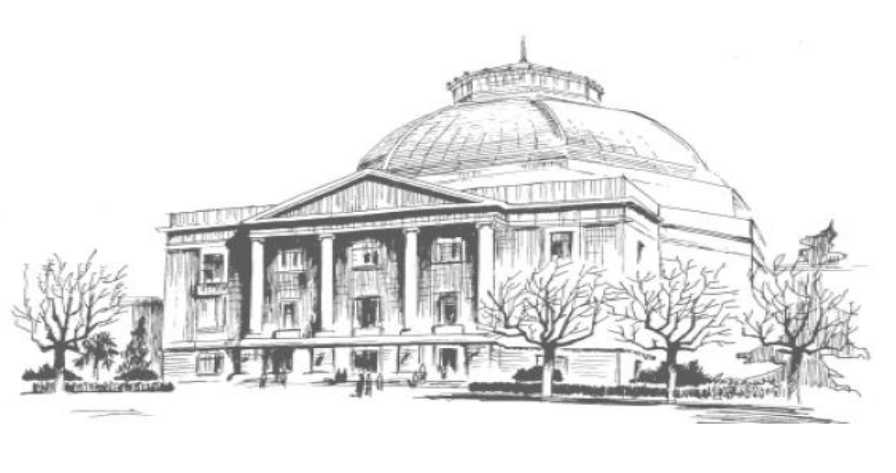
\includegraphics[width=0.9\textwidth]{pics/cover.png} \\[2pt]
        \textsc{\Huge Principles of Compilers}\\[10pt]
        \begin{tabular}[c]{rc}
            Title       & \blankToFill{\thetitle} \\
            Date        & \blankToFill{\today} \\
            Author      & \blankToFill{\theauthor\footnotemark} \\
            Student ID  & \blankToFill{\thestudentID} \\
            Institution & \blankToFill{\theinstitution}
        \end{tabular}
        \rmfamily
    \end{center}
    \footnotetext{\theemail}
\end{titlepage}}

\newcommand{\red}[1]{{\color{red}#1}}

\begin{document}
    \makecover

    \tableofcontents

    \newpage
    \section{T 3.3.5}

    Write regular definitions for the following languages:

    \begin{enumerate} 
        \item[(a)] All strings of lowercase letters that contain the five vowels in order;
        \item[(b)] All strings of lowercase letters in which the letters are in ascending lexicographic order;
        \item[(c)] Comments, consisting of a string surrounded by \verb|/*| and \verb|*/|, without an intervening \verb|*/|, unless it is inside double-quotes \verb|"|;
        \item[(h)] All strings of \verb|a|'s and \verb|b|'s that do not contain the substring \verb|abb|;
        \item[(i)] All strings of \verb|a|'s and \verb|b|'s that do not contain the subsequence \verb|abb|;
    \end{enumerate}

    \textbf{Solutions}:
    \begin{enumerate}
        \item[(a)] The DFA that represents the language is shown in the figure \ref{fig:t1-a}.
        
        Then we can get the regular grammar as below:
        \begin{gather*}
            S \to others^*\;\mathrm{a}\;(\mathrm{a}|others)^*\;\mathrm{e}\;(\mathrm{e}|others)^*\;\mathrm{i}\;(\mathrm{i}|others)^*\;\mathrm{o}\;(\mathrm{o}|others)^*\;\mathrm{u}\;(\mathrm{u}|others)^* \\
            others \to [\mathrm{a}-\mathrm{z}]\backslash\{\mathrm{a,e,i,o,u}\}
        \end{gather*}
        \item[(b)] The regular grammar is shown below:
        \[
            S \to \mathrm{a}^*\;\mathrm{b}^*\;\mathrm{c}^*\ldots\mathrm{z}^*
        \]
        \item[(c)] The FA represents the language is shown in the figure \ref{fig:t1-c}.
        
        From the FA we can get the regular grammar:
        \begin{align*}
            L &\to /*((*^*|others)\;|\;"(others|*|/)^*")^**^+/ \\
            others &\to S \backslash\{/,*,"\}
        \end{align*}
        \item[(h)] $S \to \mathrm{b}^*(\mathrm{ab}^?)^*$
        \item[(i)] $S \to \mathrm{b}^*(\mathrm{a}^+\mathrm{b}^?\mathrm{a}^*)^?$
    \end{enumerate}

    \begin{figure}[hp]
        \centering
        \begin{dot2tex}[scale=0.85]
        digraph {
            node[shape="circle"];
            rankdir="LR";
            S[shape="point",label="start"];
            F[shape="doublecircle"]
            S -> A [label="start"];
            A -> A [label="others"]
            A -> B [label="a"];
            B -> B [label="[a]|others"];
            B -> C [label="e"];
            C -> C [label="[e]|others"];
            C -> D [label="i"];
            D -> D [label="[i]|others"];
            D -> E [label="o"];
            E -> E [label="[o]|others"];
            E -> F [label="u"];
            F -> F [label="[u]|others"]
        }
        \end{dot2tex}
        \caption{DFA that represents the language in (a)}
        \label{fig:t1-a}
    \end{figure}

    \begin{figure}[hp]
        \centering
        \begin{dot2tex}[scale=1]
        digraph {
            node [shape="circle"];
            rankdir = "LR";
            S [shape="point",label="start"];
            E [shape="doublecircle"]
            S -> A [label="start"];
            A -> B [label="/"];
            B -> C [label="*"]
            C -> C [label="others"];
            C -> D [label="*"];
            D -> D [label="*"];
            D -> C [label="others"];
            D -> E [label="/"];
            C -> F [label="\""]
            F -> F [label="others|*|/"]
            F -> C [label="\""];
        }
        \end{dot2tex}
        \caption{FA that represents the language in (c)}
        \label{fig:t1-c}
    \end{figure}

    \clearpage
    \newpage
    \section{T 3.9.3}

    We can prove that two regular expressions are equivalent by showing that their minimum-state DFA’s are the same up to renaming of states. Show in this way that the following regular expressions: $(\mathrm{a|b})^*$, $(\mathrm{a^*|b^*})^*$, and $(\mathrm{(\varepsilon|a)b^*})^*$ are all equivalent. 

    \begin{proof}
        The minimum-state DFA of regular expression $(\mathrm{a|b})^*$ is shown in figure \ref{fig:t2-1}.

        The NFA of regular expression $(\mathrm{a^*|b^*})^*$ is shown in figure \ref{fig:t2-2-1}, and by applying the transition table shown in table \ref{fig:t2-2-tab}, we can get its minimum-state DFA in figure \ref{fig:t2-2-2}.

        The NFA of regular expression $(\mathrm{(\varepsilon|a)b^*})^*$ is shown in figure \ref{fig:t2-3-1}, and by applying the transition table shown in table \ref{fig:t2-3-tab}, we can get its DFA in figure \ref{fig:t2-3-2}. By simplifying \ref{fig:t2-3-2}, we get the minimum-state DFA in figure \ref{fig:t2-3-3}.

        By comparing figure \ref{fig:t2-1}, figure \ref{fig:t2-2-2} and figure \ref{fig:t2-3-3}, we can find that they're the same, after renaming state A to state 1 in figure \ref{fig:t2-1}. So the given three regular expressions are equivalent.
    \end{proof}

    \begin{figure}[hp]
        \centering
        \begin{dot2tex}[scale=1]
            digraph {
                node [shape="circle"];
                rankdir = "LR";
                S [shape="point",label="start"];
                A [shape="doublecircle"];
                S -> A [label="start"];
                A:n -> A:n [label="a"];
                A:s -> A:s [label="b"];
            }
        \end{dot2tex}
        \caption{minimum-state DFA of regular expression $(\mathrm{a|b})^*$}
        \label{fig:t2-1}
    \end{figure}

    \begin{figure}[hp]
        \centering
        \subfloat[NFA of regular expression $(\mathrm{a^*|b^*})^*$]{
            \label{fig:t2-2-1}
            \begin{tikzpicture}[rounded corners,node distance=2cm,on grid,auto]
                \node[state,initial]    (A)                         {$A$};
                \node[state]            (B)     [right of=A]        {$B$};
                \node[state]            (C_1)   [above right of=B]  {$C_1$};
                \node[state]            (C_2)   [below right of=B]  {$C_2$};
                \node[state]            (D_1)   [right of=C_1]      {$D_1$};
                \node[state]            (D_2)   [right of=C_2]      {$D_2$};
                \node[state]            (E_1)   [right of=D_1]      {$E_1$};
                \node[state]            (E_2)   [right of=D_2]      {$E_2$};
                \node[state]            (F)     [below right of=E_1]{$F$};
                \node[state,accepting]  (G)     [right of=F]        {$G$};

                \path[->]   (A)     edge                node        {$\varepsilon$} (B)
                                    edge [bend right=45]node        {$\varepsilon$} (G)
                            (B)     edge                node        {$\varepsilon$} (C_1)
                                    edge                node        {$\varepsilon$} (C_2)
                            (C_1)   edge                node        {$\varepsilon$} (D_1)
                            (C_2)   edge                node        {$\varepsilon$} (D_2)
                            (D_1)   edge                node        {$\varepsilon$} (E_1)
                                    edge [loop above]   node        {a}             ()
                            (D_2)   edge                node        {$\varepsilon$} (E_2)
                                    edge [loop above]   node        {b}             ()
                            (E_1)   edge                node        {$\varepsilon$} (F)
                            (E_2)   edge                node        {$\varepsilon$} (F)
                            (F)     edge                node        {$\varepsilon$} (G)
                                    edge [bend right=20]node        {$\varepsilon$} (B);
            \end{tikzpicture}
        } \\
        \subfloat[Transition table for the NFA]{
            \label{fig:t2-2-tab}
            \begin{tabular}{c|c|c|c}
                \hline
                NFA State & DFA State & a & b \\ \hline
                $\{A, B, C_1, C_2, D_1, D_2, E_1, E_2, F, G\}$ & 1 & 1 & 1 \\ \hline
            \end{tabular}
        }\\
        \subfloat[minimum-state DFA of regular expression $(\mathrm{a^*|b^*})^*$]{
            \makebox[0.9\textwidth]{
                \begin{tikzpicture}[rounded corners,node distance=2cm,on grid,auto]
                    \node[initial,state,accepting]  (A) {1};
    
                    \path[->]   (A) edge [loop above]   node    {a} ()
                                    edge [loop below]   node    {b} ();
                \end{tikzpicture}
            }
            \label{fig:t2-2-2}
        }
        \caption{FAs of regular expression $(\mathrm{a^*|b^*})^*$}
        \label{fig:t2-2}
    \end{figure}

    \begin{figure}[hp]
        \centering
        \subfloat[NFA of regular expression $(\mathrm{(\varepsilon|a)b^*})^*$]{
            \label{fig:t2-3-1}
            \begin{tikzpicture}[rounded corners,node distance=1.5cm,on grid,auto,nodes={ scale=.8}]
                \node[state,initial]    (A)                         {$A$};
                \node[state]            (B)     [right of=A]        {$B$};
                \node[state]            (C_1)   [above right of=B]  {$C_1$};
                \node[state]            (C_2)   [below right of=B]  {$C_2$};
                \node[state]            (D_1)   [right of=C_1]      {$D_1$};
                \node[state]            (D_2)   [right of=C_2]      {$D_2$};
                \node[state]            (E)     [below right of=D_1]{$E$};
                \node[state]            (F)     [right of=E]        {$F$};
                \node[state]            (G)     [right of=F]        {$G$};
                \node[state]            (H)     [right of=G]        {$H$};
                \node[state,accepting]  (I)     [right of=H]        {$I$};

                \path[->]   (A)     edge                node        {$\varepsilon$} (B)
                                    edge [bend right=45]node        {$\varepsilon$} (I)
                            (B)     edge                node        {$\varepsilon$} (C_1)
                                    edge                node        {$\varepsilon$} (C_2)
                            (C_1)   edge                node        {a} (D_1)
                            (C_2)   edge                node        {$\varepsilon$} (D_2)
                            (D_1)   edge                node        {$\varepsilon$} (E)
                            (D_2)   edge                node        {$\varepsilon$} (E)
                            (E)     edge                node        {$\varepsilon$} (F)
                            (F)     edge                node        {$\varepsilon$} (G)
                            (G)     edge                node        {$\varepsilon$} (H)
                                    edge [loop above]   node        {b}             ()
                            (H)     edge                node        {$\varepsilon$} (I)
                                    edge [bend right=80]node        {$\varepsilon$} (B);
            \end{tikzpicture}
        } \\
        \subfloat[Transition table for the NFA]{
            \label{fig:t2-3-tab}
            \begin{tabular}{c|c|c|c}
                \hline
                NFA State & DFA State & a & b \\ \hline
                $\{A, B, C_1, C_2, D_2, F, G, H, I\}$ & 1 & 2 & 1 \\ \hline
                $\{A, B, C_1, C_2, D_1, D_2, F, G, H, I\}$ & 2 & 2 & 1 \\ \hline
            \end{tabular}
        }\\
        \subfloat[DFA of regular expression $(\mathrm{(\varepsilon|a)b^*})^*$]{
            \makebox[0.9\textwidth]{
                \begin{tikzpicture}[rounded corners,node distance=2cm,on grid,auto]
                    \node[initial,state,accepting]  (A)                 {1};
                    \node[state,accepting]          (B) [right of=A]    {2};
    
                    \path[->]   (A) edge [bend right=40]node    {a} (B)
                                    edge [loop above]   node    {b} ()
                                (B) edge [loop above]   node    {a} ()
                                    edge [bend right=40]node    {b} (A);
                \end{tikzpicture}
            }
            \label{fig:t2-3-2}
        }\\
        \subfloat[minimum-state DFA of regular expression $(\mathrm{(\varepsilon|a)b^*})^*$]{
            \makebox[0.9\textwidth]{
                \begin{tikzpicture}[rounded corners,node distance=2cm,on grid,auto]
                    \node[initial,state,accepting]  (A) {1};
    
                    \path[->]   (A) edge [loop above]   node    {a} ()
                                    edge [loop below]   node    {b} ();
                \end{tikzpicture}
            }
            \label{fig:t2-3-3}
        }
        \caption{FAs of regular expression $(\mathrm{(\varepsilon|a)b^*})^*$}
        \label{fig:t2-3}
    \end{figure}

    \clearpage
    \newpage
    \section{Language to FA then to linear grammar}

    $L = \{\omega | \omega\in(\mathrm{a}|\mathrm{b})^*$ with an odd number of a's and an even number of b's and that begins with a and ends with b.$\}$. Please

    \begin{enumerate}
        \item construct a FA to recognize $L$;
        \item and then translate the FA into right linear grammar and left linear grammar;
        \item eliminate the $\varepsilon$ productions in the grammar you just got.
    \end{enumerate}

    \textbf{Solutions}:

    \begin{enumerate}
        \item The FA should starts with an a and ends with a b. So we can construct a skeleton of the FA as in figure \ref{fig:t3-1-1}, where the \red{???} should be completed later.
        
        Then consider how to complete the \red{???}. We need 4 states (includeing $B$ and $C$ in figure \ref{fig:t3-1-1}), to represent the state of a's and b's count, as shown in table \ref{fig:t3-1-trans}. With the table, a completed NFA can be constructed as figure \ref{fig:t3-1-2} shows.
        \item The left linear grammar:
        \begin{align*}
            T &\to C\mathrm{b} \\
            C &\to B\mathrm{b}\;|\;E\mathrm{a} \\
            B &\to A\mathrm{a}\;|\;C\mathrm{b}\;|\;D\mathrm{a} \\
            D &\to B\mathrm{a}\;|\;E\mathrm{b} \\
            E &\to D\mathrm{b}\;|\;C\mathrm{a} \\
            A &\to \varepsilon
        \end{align*}
        The right linear grammar:
        \begin{align*}
            A &\to \mathrm{a}B \\
            B &\to \mathrm{b}C\;|\;\mathrm{a}D \\
            C &\to \mathrm{b}T\;|\;\mathrm{b}B\;|\;\mathrm{a}E \\
            D &\to \mathrm{a}B\;|\;\mathrm{b}E \\
            E &\to \mathrm{a}C\;|\;\mathrm{b}D \\
            T &\to \varepsilon
        \end{align*}
        \item The left linear grammar:
        \begin{align*}
            T &\to C\mathrm{b} \\
            C &\to B\mathrm{b}\;|\;E\mathrm{a} \\
            B &\to \mathrm{a}\;|\;C\mathrm{b}\;|\;D\mathrm{a} \\
            D &\to B\mathrm{a}\;|\;E\mathrm{b} \\
            E &\to D\mathrm{b}\;|\;C\mathrm{a}
        \end{align*}
        The right linear grammar:
        \begin{align*}
            A &\to \mathrm{a}B \\
            B &\to \mathrm{b}C\;|\;\mathrm{a}D \\
            C &\to \mathrm{b}\;|\;\mathrm{b}B\;|\;\mathrm{a}E \\
            D &\to \mathrm{a}B\;|\;\mathrm{b}E \\
            E &\to \mathrm{a}C\;|\;\mathrm{b}D \\
        \end{align*}
    \end{enumerate}

    \begin{figure}[hp]
        \centering
        \subfloat[The FA skeleton]{
            \begin{tikzpicture}[rounded corners,node distance=2cm,on grid,auto]
                \node[initial,state]    (A)                 {$A$};
                \node[state]            (B) [right of=A]    {$B$};
                \node[state]            (C) [right of=B]    {$C$};
                \node[state,accepting]  (D) [right of=C]    {$T$};

                \path[->]   (A) edge    node    {a} (B)
                            (C) edge    node    {b} (D);
                \path[-,dashed,red]    (B) edge    node    {???}   (C);
            \end{tikzpicture}
            \label{fig:t3-1-1}
        } \\
        \subfloat[The states in the \red{???} part]{
            \begin{tabular}{lcccc}
                \toprule
                 & \multicolumn{2}{c}{Count of characters} & \multicolumn{2}{c}{State transition} \\ \cmidrule(l{.2em}r{.2em}){2-3} \cmidrule(l{.2em}r{.2em}){4-5}
                 & a & b & a & b \\ \midrule
                $B$ & odd & even & $D$ & $C$ \\
                $D$ & even & even & $B$ & $E$ \\
                $E$ & even & odd & $C$ & $D$ \\
                $C$ & odd & odd & $E$ & $\{T, B\}$ \\
                \bottomrule
            \end{tabular}
            \label{fig:t3-1-trans}
        } \\
        \subfloat[The completed NFA]{
            \begin{tikzpicture}[rounded corners,node distance=1.8cm,auto,nodes={scale=0.8}]
                \node[initial,state]    (A)                 {$A$};
                \node[state]            (B) [right of=A]    {$B$};
                \node[state]            (C) [right of=E]    {$C$};
                \node[state]            (D) [right of=B]    {$D$};
                \node[state]            (E) [right of=D]    {$E$};
                \node[state,accepting]  (T) [right of=C]    {$T$};

                \path[->]   (A) edge                    node    {a} (B)
                            (B) edge [bend right=40]    node    {a} (D)
                                edge [bend right=60]    node    {b} (C)
                            (D) edge [bend right=40]    node    {a} (B)
                                edge [bend right=40]    node    {b} (E)
                            (E) edge [bend right=40]    node    {a} (C)
                                edge [bend right=40]    node    {b} (D)
                            (C) edge                    node    {b} (T)
                                edge [bend right=60]    node    {b} (B)
                                edge [bend right=40]    node    {a} (E);
            \end{tikzpicture}
            \label{fig:t3-1-2}
        } 
        \caption{FAs of T3}
        \label{fig:t3-1}
    \end{figure}
\end{document}
